% !TEX root = ../ppt.tex


% 目录页
\begin{frame}{目录}
    \begin{itemize}
        \item 高斯过程
        \begin{itemize}
            \item[-] 单变量高斯分布
            \item[-] 多维高斯分布(性质)
            \item[-] 高斯过程(均值函数与协方差函数)
        \end{itemize}

        \item 高斯过程回归模型
        \begin{itemize}
            \item[-] 统计模型优劣
            \item[-] 模型建立
            \item[-] 模型求解
        \end{itemize}

        \item 高斯过程回归模型应用
        \begin{itemize}
            \item[-] 仿真
            \item[-] 大气$CO_{2}$浓度预测
        \end{itemize}

        \item 参考
    \end{itemize}
\end{frame}

% ------------------------- 高斯过程 -------------------------------

% 1
\begin{frame}[fragile]{高斯过程}
    \begin{definition}[高斯分布]
        \vspace{2ex}
        一个连续型随机变量$X$其概率密度函数(probability density function, pdf)若为
        
        \begin{equation}
            f(x)=\frac{1}{\sqrt{2\pi}\sigma}\mathrm{exp}\left(-\frac{(x-\mu)^2}{2\sigma^{2}}\right)\qquad x\in \mathds{R}. 
        \end{equation}

        其中$\mu\in\mathds{R}$, $\sigma^{2}\geqslant 0$, 则称$X$服从均值为$\mu$方差为$\sigma^{2}$的高斯分布(Gaussian distribution)或正态分布(normal distribution). 记作
        $$X\sim\mathcal{N}(\mu, \sigma^{2})$$
    \end{definition}
\end{frame}

% 2
\begin{frame}[fragile]{高斯过程}
    随机变量的概念很容易推广到多维随机变量(multivariate random variables)或称为随机向量(random vectors). 

    $$Y=(Y_{1},\dots,Y_{d})^{T}$$

    $Y$每一个分量都是定义在{\bf 同一个概率空间}下的随机变量. 随机向量$Y$的一个样本$y$应有$y\in\mathds{R}^{d}$.
    
    \begin{align}
        &\mathrm{E}(Y)=(\mathrm{E}(Y_{1}),\dots,\mathrm{E}(Y_{d}))^{T}. \\
        &\mathrm{var}(Y)=\mathrm{E}(YY^{T})-\mathrm{E}(Y)\mathrm{E}(Y^{T})=\mathrm{E}[(Y-\mathrm{E}(Y))(Y-\mathrm{E}(Y))^{T}]. \\
        &\mathrm{cov}(Y, Z)=\mathrm{E}(YZ^{T})-\mathrm{E}(Y)\mathrm{E}(Z^{T}).
    \end{align}

\end{frame}

% 3
\begin{frame}[fragile]{高斯过程}
    \begin{definition}[多维高斯分布] 
        \vspace{2ex}     
        若有随机向量$Y=(Y_{1},\dots,Y_{d})^{T}$, 其分量的任意线性组合而成的{\bf 随机变量}都服从于高斯分布, 即
        \begin{equation}
            \forall\alpha\in\mathds{R}^{d},\ \alpha_{1}Y_{1}+\dots+\alpha_{d}Y_{d}=\alpha^{T}Y\sim\mathcal{N}.
        \end{equation}
        此时称随机向量$Y$服从于$d$维高斯分布, $Y$也被称为高斯随机向量.
    \end{definition}

    $d$维高斯分布的概率密度函数由下式给出.

    \begin{equation}
        f_{Y}(y)=\frac{1}{|2\pi\Sigma|^{1/2}}\mathrm{exp}\left(-\frac{1}{2}(y-\mu)^{T}\Sigma^{-1}(y-\mu)\right) \qquad y\in\mathds{R}^{d}. \label{2.6}
    \end{equation}

    可简记为,
    \begin{equation}
        Y \sim f(y)=\mathcal{N}(\mu, \Sigma)
    \end{equation}

\end{frame}

% 4
\begin{frame}[fragile]{高斯过程}
    \begin{equation*}
        f_{Y}(y)=\frac{1}{|2\pi\Sigma|^{1/2}}\mathrm{exp}\left(-\frac{1}{2}(y-\mu)^{T}\Sigma^{-1}(y-\mu)\right) \qquad y\in\mathds{R}^{d}. 
    \end{equation*}

    \begin{equation*}
        Y \sim f(y)=\mathcal{N}(\mu, \Sigma)
    \end{equation*}

    其中$\mu$是$d$维的均值向量(mean vector), 其每个分量$\mu_{i}=\mathrm{E}(Y_{i})$,而$\Sigma$是一个$d\times d$的矩阵, 其$i$行$j$列的分量$\Sigma_{i,j}=\mathrm{cov}(Y_{i},Y_{j})$, 矩阵$\Sigma$被称为协方差矩阵(covariance matrix).

    多维高斯分布的特性由均值向量$\mu$与协方差矩阵$\Sigma$唯一确定. 可以证明但此处不证, 协方差矩阵总是对称半正定(symmetric and positive semi-definite)的, 即,

    \begin{align}
        &\Sigma_{i,j}=\Sigma_{j,i}. \\
        &\forall\alpha\in\mathds{R}^{d},\ \alpha^{T}\Sigma\alpha\geqslant 0.
    \end{align}
\end{frame}

% 5
\begin{frame}[fragile]{高斯过程}
    \begin{property}
        对于高斯向量来说, 各分量之间不相关等价于各分量之间独立.
    \end{property}

    \begin{equation}
        \Sigma= \begin{pmatrix}
                    \sigma^{2}_{1} & 0 & \cdots & 0 \\
                    0 & \sigma^{2}_{2} & \cdots & 0 \\ 
                    \vdots & \vdots & \ddots & \vdots \\
                    0 & 0 & \cdots & \sigma^{2}_{d} \\
                \end{pmatrix}
    \end{equation}

    \begin{align}
        f(y)&=\frac{1}{|2\pi\Sigma|^{1/2}}\mathrm{exp}\left(-\frac{1}{2}(y-\mu)^{T}\Sigma^{-1}(y-\mu)\right) \notag \\
        &=\frac{1}{\sqrt{2\pi\sigma^{2}_{1}}\times \dots\times\sqrt{2\pi\sigma^{2}_{d}}} \mathrm{exp}\left(-\sum^{d}_{i=1}\frac{(y_{i}-\mu_{i})^{2}}{2\sigma^{2}_{i}}\right) \notag \\
        &=\prod^{d}_{i=1}f(y_{i}).
    \end{align}    

\end{frame}

% 6
\begin{frame}[fragile]{高斯过程}
    $$Y \sim f(y)=\mathcal{N}(\mu, \Sigma)$$
    为了研究高斯分布的条件分布, 我们把高斯随机向量划分为两部分, $Y=\left( {Y_{1}\atop Y_{2}}\right)$, $Y_{1}$与$Y_{2}$都可能为高斯随机向量或只是单变量(univariate). 同时也对应将均值向量与协方差矩阵分块,
    \begin{align}
        &\mu=   \begin{pmatrix}
                        \mu_{1} \\ \mu_{2} \\
                \end{pmatrix}  \\
        &\Sigma=\begin{pmatrix}\label{2.13}
                    \Sigma_{1,1} & \Sigma_{1,2} \\
                    \Sigma_{2,1} & \Sigma_{2,2} \\
                \end{pmatrix}
    \end{align}
\end{frame}

% 7
\begin{frame}[fragile]{高斯过程}
    \begin{property}
        已知$Y_{2}$的条件下$Y_{1}$的条件分布也是高斯分布. 若$Y_{1}$为随机向量, 则该条件分布是多维高斯分布, 且该多维高斯分布的均值向量与协方差函数由下式给出,
        \begin{align}
            &Y_{1}|Y_{2}\sim\mathcal{N}(\mu_{c}, \Sigma_{c}). \notag \\
            &\mu_{c}=\mu_{1}+\Sigma_{1,2}\Sigma_{2,2}^{-1}(Y_{2}-\mu_{2}). \\
            &\Sigma_{c}=\Sigma_{1,1}-\Sigma_{1,2}\Sigma^{-1}_{2,2}\Sigma_{2,1}.
        \end{align}
    \end{property}

    其中$Y=\left( {Y_{1}\atop Y_{2}}\right)$, $\mu=\left( {\mu_{1}\atop \mu_{2}}\right)$, $\Sigma=\left({\Sigma_{1,1} \ \Sigma_{1,2}\atop   \Sigma_{2,1} \ \Sigma_{2,2}} \right)$.
\end{frame}

% 8
\begin{frame}[fragile]{高斯过程}
    分块矩阵求逆定理(inversion of a partitioned matrix). 设矩阵$A$为分块矩阵, 其逆阵为$A^{-1}$,

    \begin{equation}
        A=  \begin{pmatrix}
                P & Q \\
                R & S \\
            \end{pmatrix}, \qquad\qquad
        A^{-1}= \begin{pmatrix}
                    \tilde{P} & \tilde{Q} \\
                    \tilde{R} & \tilde{S} \\
                \end{pmatrix}.
    \end{equation}

    其中$P$与$\tilde{P}$为$n_{1}\times n_{1}$的方阵, $S$与$\tilde{S}$为$n_{2}\times n_{2}$的方阵. 在已知$P$,$Q$,$R$,$S$的条件下, 可由下式计算得到$\tilde{P}$,$\tilde{Q}$,$\tilde{R}$,$\tilde{S}$.

    \begin{equation}
        \begin{cases}
            \tilde{P}=N. \\
            \tilde{Q}=-NQS^{-1}. \\ 
            \tilde{R}=-S^{-1}RN. \\
            \tilde{S}=S^{-1}+S^{-1}RNQS^{-1}.
        \end{cases}
    \end{equation}

    其中$N=(P-QS^{-1}R)^{-1}$.
\end{frame}

% 9
\begin{frame}[fragile]{高斯过程}
    \textbf{证明:}不失一般性, 我们假定$Y$是经过中心化的, 即$\mu=0$. 对于高斯分布我们通常只需关注指数部分, 从多维高斯分布的pdf出发,我们得到,
    \begin{align}\label{A2.7}
        f_{Y}(y)&\propto\mathrm{exp}\left(-\frac{1}{2}y^{T}\Sigma^{-1}y\right) \notag \\
        &\propto\mathrm{exp}\left( -\left(y^{T}_{1}\ y^{T}_{2}\right)
        \begin{pmatrix}
            \Sigma_{1,1} & \Sigma_{1,2} \\
            \Sigma_{2,1} & \Sigma_{2,2} \\
        \end{pmatrix}^{-1}
        \left({y_{1}\atop y_{2}}\right)\right).
    \end{align}

    下面求分块矩阵的逆,令,

    \begin{equation}
        \begin{pmatrix}
            \Sigma_{1,1} & \Sigma_{1,2} \\
            \Sigma_{2,1} & \Sigma_{2,2} \\
        \end{pmatrix}^{-1}=
        \begin{pmatrix}
            A & B \\
            C & D \\
        \end{pmatrix}.
    \end{equation}
\end{frame}

% 10
\begin{frame}[fragile]{高斯过程}
    由分块矩阵求逆定理及协方差矩阵性质$\Sigma_{1,2}=\Sigma^{T}_{2,1}$可求得, 
    \begin{equation}
        \begin{cases}
            A=N. \\
            B=-N\Sigma_{1,2}\Sigma_{2,2}^{-1}. \\ 
            C=-\Sigma_{2,2}^{-1}\Sigma_{2,1}N. \\
            D=\Sigma_{2,2}^{-1}+\Sigma_{2,2}^{-1}\Sigma_{2,1}N\Sigma_{1,2}\Sigma_{2,2}^{-1}. 
        \end{cases} 
    \end{equation}

    上式中$N=(\Sigma_{1,1}-\Sigma_{1,2}\Sigma^{-1}_{2,2}\Sigma_{2,1})^{-1}$.

    \begin{align}\label{A.10}
        f_{Y}(y)&\propto\mathrm{exp}\left( -\left(y^{T}_{1}\ y^{T}_{2}\right)
        \begin{pmatrix}
            A & B \\
            C & D \\
        \end{pmatrix}
        \left({y_{1}\atop y_{2}}\right)\right)\notag\\
        &\propto\mathrm{exp}(-y^{T}_{1}Ay_{1}-y^{T}_{2}Cy_{1}-y^{T}_{1}By_{2}-y^{T}_{2}Dy_{2} )\notag \\
        &\propto\dots \\ 
        &\propto\mathrm{exp}\left(-(y_{1}-\Sigma_{1,2}\Sigma^{-1}_{2,2}y_{2})^{T}(\Sigma_{1,1}-\Sigma^{-1}_{2,2}\Sigma_{2,1})^{-1}(y_{1}-\Sigma_{1,2}\Sigma^{-1}_{2,2}y_{2})\right). \notag
    \end{align}

\end{frame}

% 11
\begin{frame}[fragile]{高斯过程}
    $$f_{Y}(y)\propto\mathrm{exp}\left(-(y_{1}-\underbrace{\Sigma_{1,2}\Sigma^{-1}_{2,2}y_{2}}_{\mu_{c}})^{T}(\underbrace{\Sigma_{1,1}-\Sigma^{-1}_{2,2}\Sigma_{2,1}}_{\Sigma_{c}})^{-1}(y_{1}-\underbrace{\Sigma_{1,2}\Sigma^{-1}_{2,2}y_{2}}_{\mu_{c}})\right).$$

    在$y_{2}$已知的条件下, $\mu_{c}=\Sigma_{1,2}\Sigma^{-1}_{2,2}y_{2}$与$\Sigma_{c}=\Sigma_{1,1}-\Sigma^{-1}_{2,2}\Sigma_{2,1}$是确定的, 故$Y_{1}|Y_{2}$服从均值为$\mu_{c}$,协方差矩阵为$\Sigma_{c}$的高斯分布, 即

    $$Y_{1}|Y_{2}\sim\mathcal{N}(\mu_{c},\Sigma_{c}).$$

    如果不考虑进行中心化, 则只需将$y_{1}$与$y_{2}$分别用$y_{1}-\mu_{1}$与$y_{2}-\mu_{2}$替代, 即得到结果,
    \begin{align*}
        &\mu_{c}=\mu_{1}+\Sigma_{1,2}\Sigma_{2,2}^{-1}(Y_{2}-\mu_{2}). \\
        &\Sigma_{c}=\Sigma_{1,1}-\Sigma_{1,2}\Sigma^{-1}_{2,2}\Sigma_{2,1}.
    \end{align*}
    \rightline{$\square$} % 造一个证明完毕的符号 >_<
\end{frame}

% 12
\begin{frame}[fragile]{高斯过程}
    多维随机向量的概念可以推广到随机过程(stochastic processes).

    \begin{definition}[高斯过程]
        \vspace{2ex}  
        若一个定义在域$D\in\mathds{R}^{d}$上的随机过程$Z$, 对于$\forall n\in \mathds{N},\ \forall x_{i}\in D,\ (Z(x_{1}),\dots,Z(x_{n}))$是一个高斯随机向量, 则$Z$是高斯过程(Gaussian Process, GP).
    \end{definition}

    与高斯分布类似, 高斯过程的性质可以由定义在$D$上的均值函数(mean function)与定义在$D\times D$上的协方差函数(covariance function)完全确定. 通常用$m(x)$与$k(x,x')$来表示\uline{均值函数}与\uline{协方差函数}. 
    \begin{align}
        &m(x)=\mathrm{E}(Z(x)) \\
        &k(x,x')=\mathrm{cov}(Z(x),Z(x'))
    \end{align}
    
    于是高斯过程$Z$可简记为
    \begin{equation*}
        Z\sim\mathcal{GP}\left(m(x),k(x,x')\right)
    \end{equation*}

\end{frame}

% 13
\begin{frame}[fragile]{高斯过程}
    在实际应用中总是先将数据预处理成是$0$均值的, 即使得$m(x)=0$. 这样不仅在理论推导时带来便利, 在实际运算中也提高了效率. 

    对于高斯过程的一个样本$(Z(x_{1}),\dots,Z(x_{n}))$是服从多维高斯分布的, 这个高斯分布的协方差矩阵$K$由协方差函数计算得到
    \begin{equation}
        K= \begin{pmatrix}
                    k(x_{1},x_{1}) & k(x_{1},x_{2}) & \cdots & k(x_{1},x_{n}) \\
                    k(x_{2},x_{1}) & k(x_{2},x_{2}) & \cdots & k(x_{2},x_{n}) \\
                    \vdots         & \vdots         & \ddots & \vdots \\
                    k(x_{n},x_{1}) & k(x_{n},x_{2}) & \cdots & k(x_{n},x_{n}) \\
                \end{pmatrix}
    \end{equation}
    协方差函数中存在着最终确定高斯过程的参数, 这些参数也被称为超参数(hyper-parameters).
\end{frame}

% 14
\begin{frame}[fragile]{高斯过程}
    协方差函数也被称为核函数(kernel function). 核函数形式繁多也有多种分类方法, 常见协方差函数如下,

        \begin{table}[h]
            \centering
            \caption{常见协方差函数}
            \begin{tabular}{lll}
            \hline
            \multicolumn{1}{l}{核函数}   & \multicolumn{1}{l}{表达式} & \multicolumn{1}{l}{参数} \\ \hline
            $Constant$                    &    $\sigma^{2}_{f}$      &   $\sigma^{2}_{f}$  \\
            $Linear$                      &  $\sum^{d}_{i=1}\sigma^{2}_{i}x_{i}x'_{i}$ & $\{\sigma^{2}_{1},\dots,\sigma^{2}_{d}\}$        \\
            $Polynomial$                  &  $(xx'+\sigma^{2}_{f})^{p}$ &     $\sigma^{2}_{f}$    \\
            $Squared\ Exponential$     & $\sigma^{2}_{f}\mathrm{exp}\left(-\frac{\|x-x'\|^{2}}{2l^{2}}\right)$ & $\sigma^{2}_{f},l$   \\
            $Mat\acute{e}rn$ &    $\frac{2^{1-v}}{\Gamma(v)} \left(\frac{\sqrt{2v}r}{l}\right)^{v}K_{v}\left(\frac{\sqrt{2v}r}{l}\right)$ &  $v,l$  \\
            $Exponential$  &   $\sigma^{2}_{f}\mathrm{exp}\left(-\frac{\|x-x'\|}{l}\right)$  &  $\sigma^{2}_{f},l$   \\
            $Rational\ Quadratic$ &   $\sigma^{2}_{f}\left(1+\frac{\|x-x'\|^{2}}{2\alpha l^{2}}\right)^{-\alpha}$  &  $\sigma^{2}_{f},\alpha,l$   \\ \hline
            \end{tabular}
        \end{table}
\end{frame}

%---------------------------- 高斯过程回归模型 ----------------------------

% 15
\begin{frame}[fragile]{高斯过程回归模型 - 统计模型优劣}
    \vspace{2ex}
    为什么使用统计模型(statistical modelling)?
    \vspace{2ex}
    \begin{itemize}
        \item 样本量小
        \begin{itemize}
            \item 样本不易采集(如现实世界的实验).
            \item 样本获取的成本太高(如破坏性测试, 耗时的数值仿真).
            \item ...
        \end{itemize}
    \end{itemize}
    \begin{exampleblock}{}
        \begin{center}
        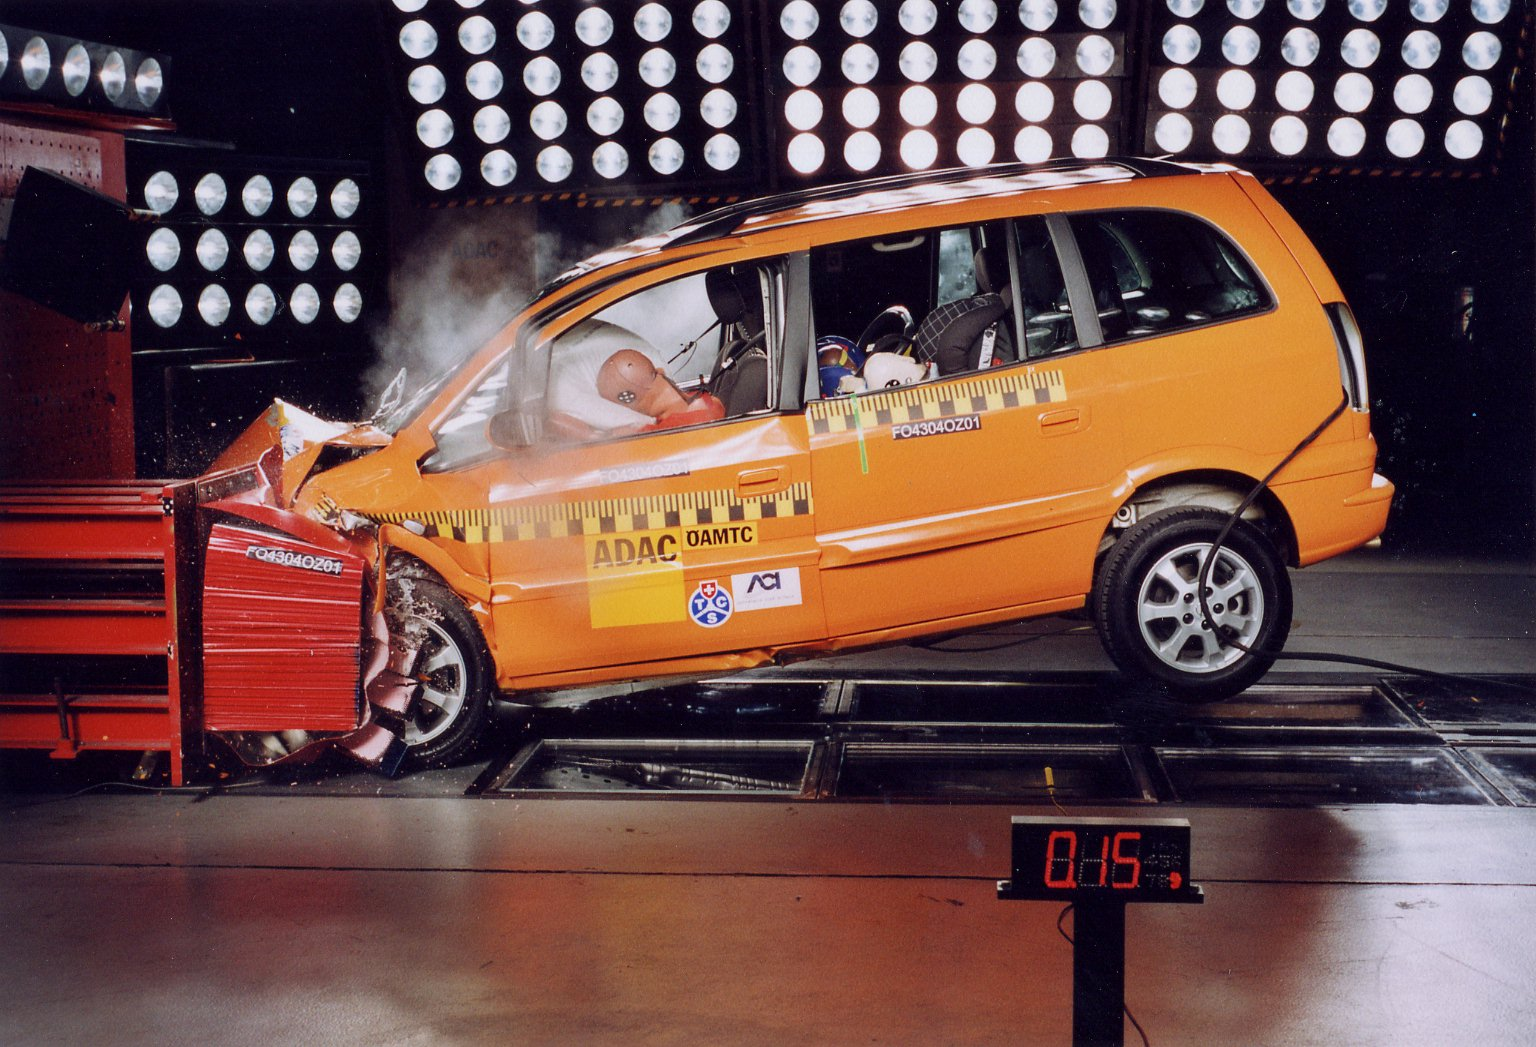
\includegraphics[height=3.5cm]{./fig/crash-test} 
        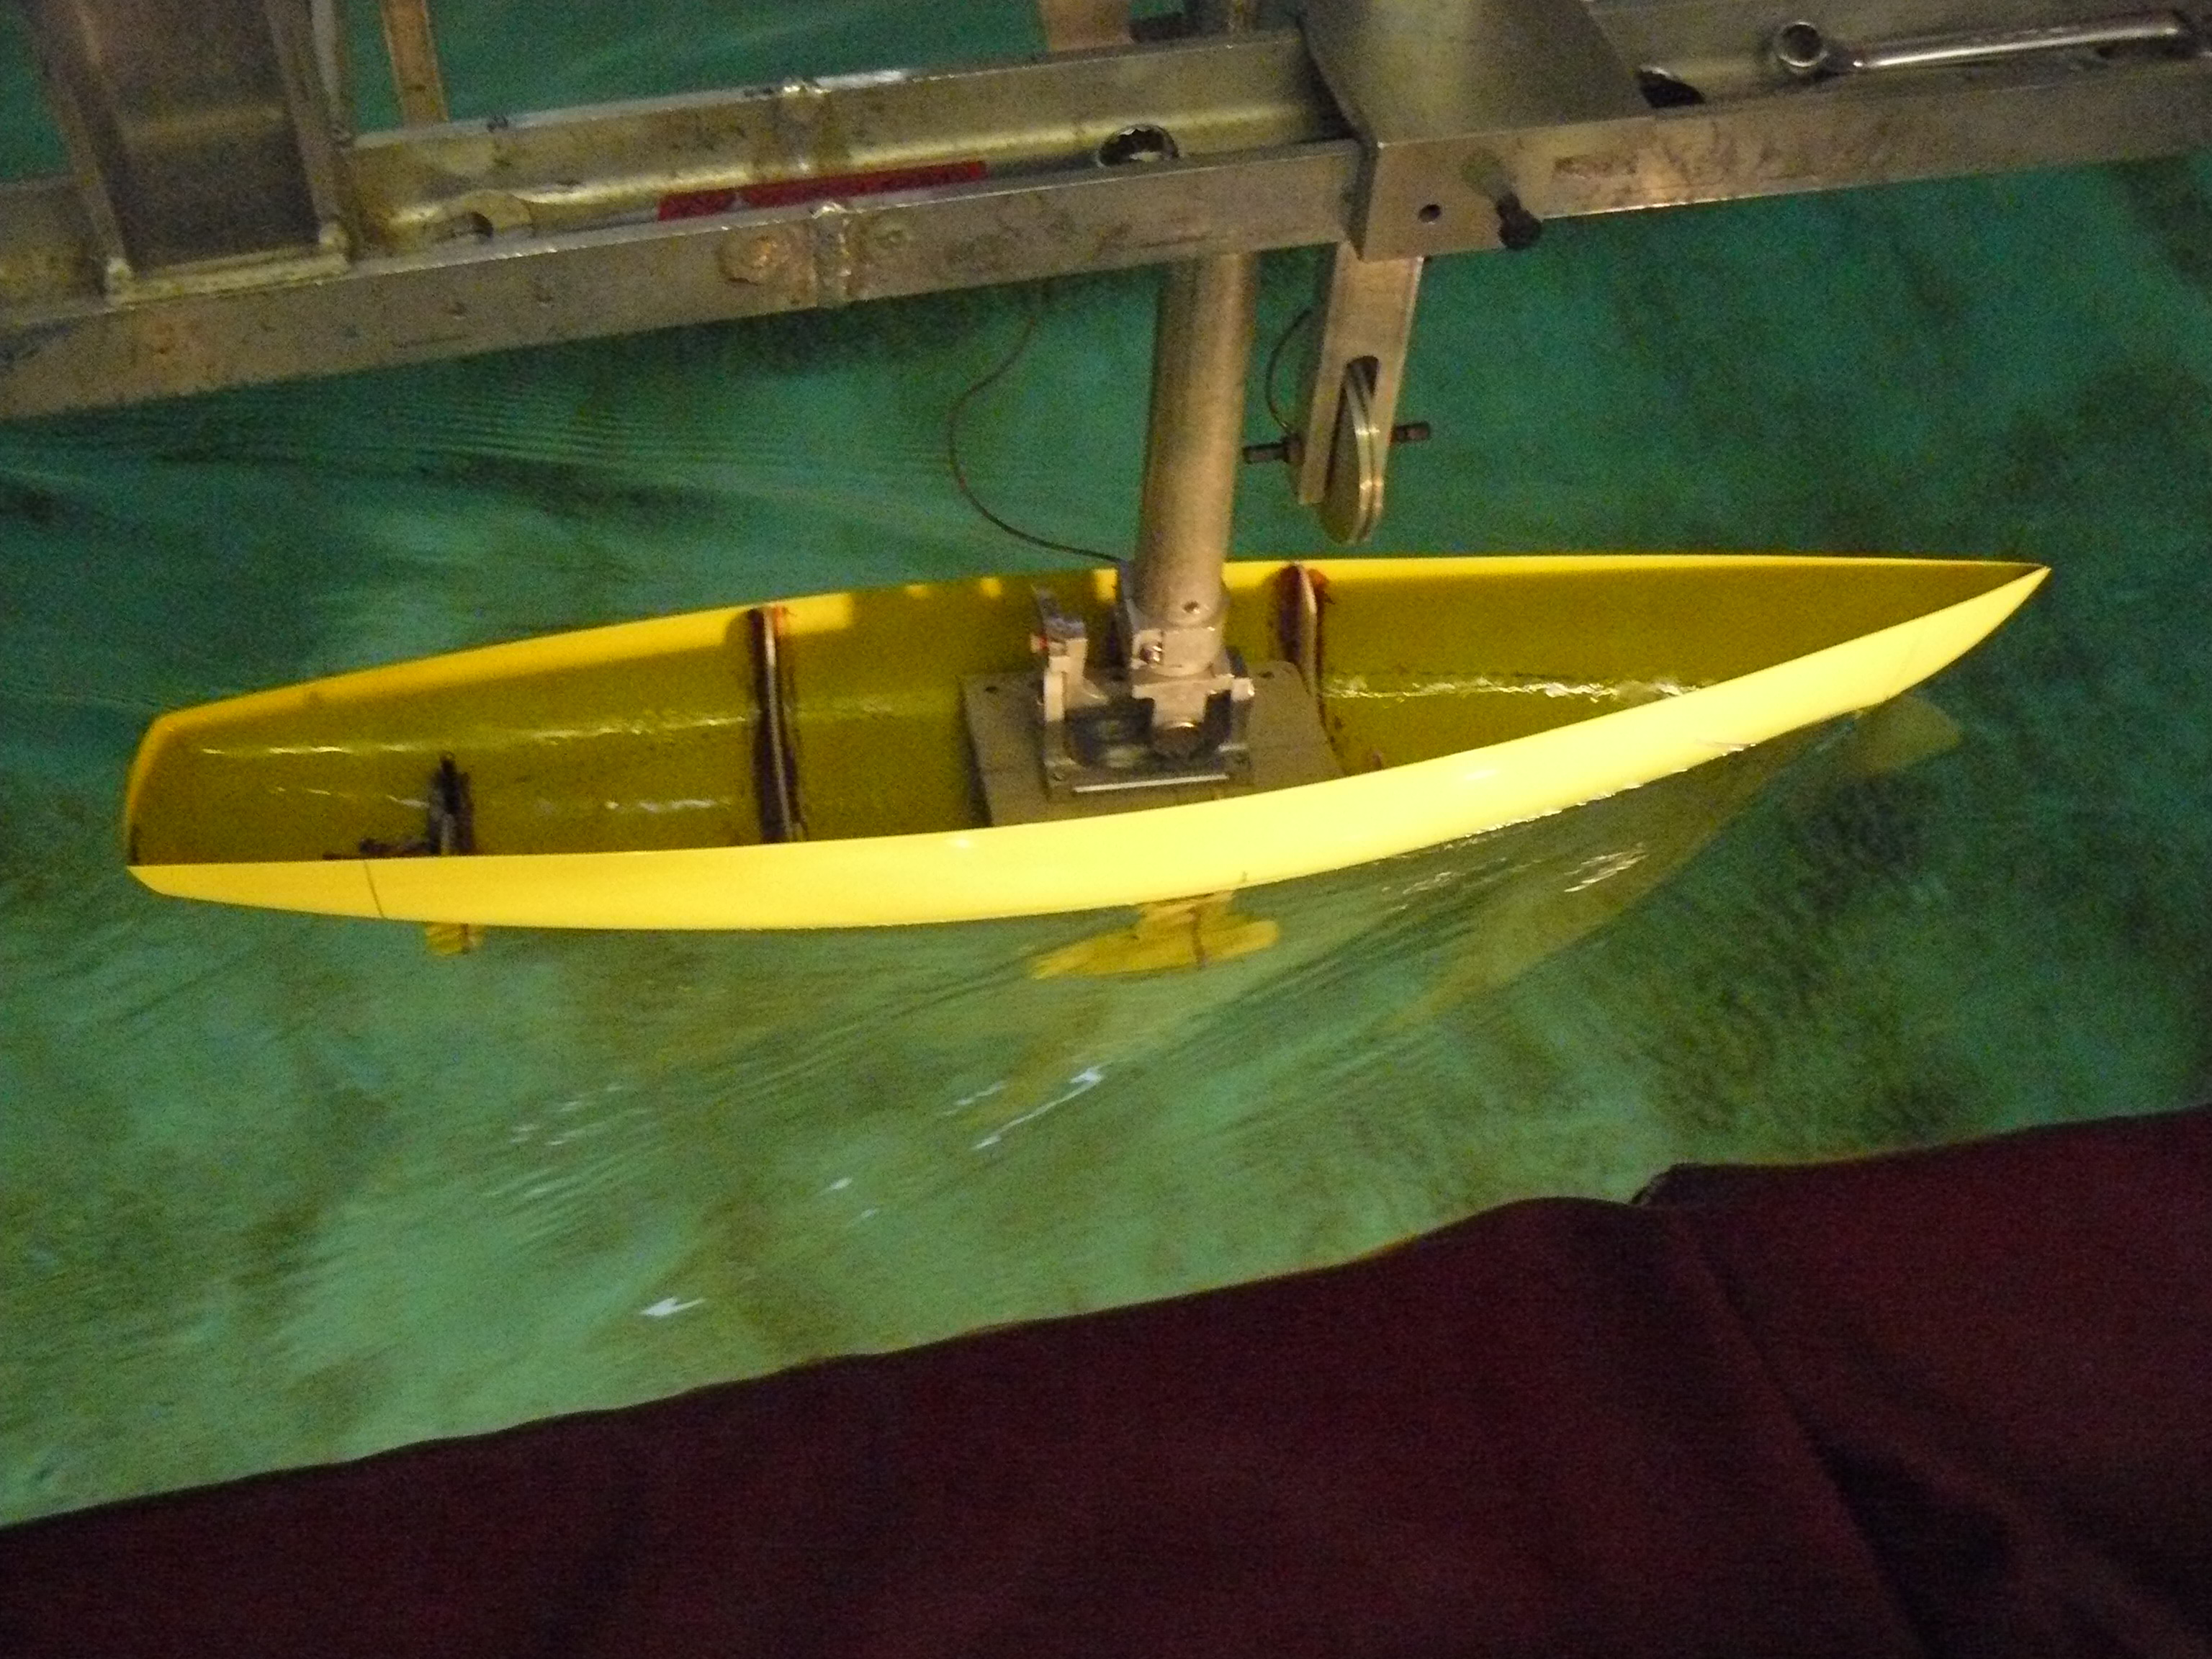
\includegraphics[height=3.5cm]{./fig/carene}
        \end{center}
    \end{exampleblock}

\end{frame}

% 16
\begin{frame}{高斯过程回归模型 - 统计模型优劣}
    \begin{itemize}
        \item 无法事先确定模型的形式.
    \end{itemize}

    \begin{center}
        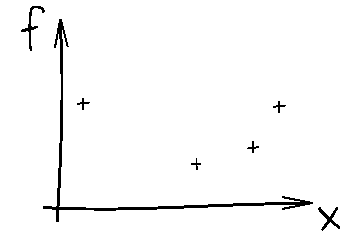
\includegraphics[height=4.5cm]{./fig/ink_fX}
    \end{center}
\end{frame}

% 17
\begin{frame}{高斯过程回归模型 - 统计模型优劣}
    \begin{itemize}
        \item 统计模型使用数据得到预测分布进行预测, 同时可给出模型误差置信区间, 量化模型预测的不确定性.
    \end{itemize}

    \begin{center}
        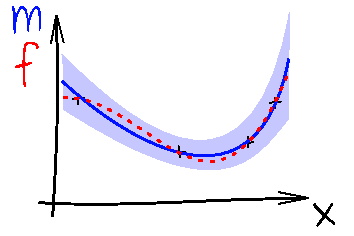
\includegraphics[height=4.5cm]{./fig/ink_mconfint}
    \end{center}
\end{frame}

% 18
\begin{frame}[fragile]{高斯过程回归模型 - 建立模型}

    模型假设
    
    $$y=f(\boldsymbol{x})+\varepsilon.$$

    假设域$D\in\mathds{R}^{d}$, $\boldsymbol{x}\in D$, $y\in\mathds{R}$, $\varepsilon\sim\mathcal{N}(0,\ \sigma^{2}_{n})$, 并设$f$是定义在$D$上的高斯过程.
        $$f\sim\mathcal{GP}\left(0, k(\boldsymbol{x},\ \boldsymbol{x}')\right).$$

    经过采样, 得到训练数据集$\{(\boldsymbol{x}_{i},y_{i})|i=1,\dots,n\}$,记$\{(\boldsymbol{X}, \boldsymbol{y})\}$. 同样可获得测试数据集$\{(\boldsymbol{X}_{*}, \boldsymbol{y}_{*})\}$.
\end{frame}

% 19
\begin{frame}[fragile]{高斯过程回归模型 - 建立模型}

    由高斯过程理论, 可知联合分布服从高斯分布.
    
    $$\left[\begin{aligned}
        \boldsymbol{y}\ \\
        \boldsymbol{f}_{*}
    \end{aligned}\right]
    \sim\mathcal{N}\left(0,\
    \begin{bmatrix}
        &K(\boldsymbol{X}, \boldsymbol{X}) + \sigma^{2}_{n}I    &K(\boldsymbol{X}, \boldsymbol{X}_{*}) \\
        &K(\boldsymbol{X}_{*}, \boldsymbol{X}) &K(\boldsymbol{X}_{*}, \boldsymbol{X}_{*})
    \end{bmatrix}\right).$$

    此处$K(\boldsymbol{X},\boldsymbol{X}')$为简记, 当$\boldsymbol{X}=(\boldsymbol{x}_{1}\dots \boldsymbol{x}_{m})$与$\boldsymbol{X}'=(\boldsymbol{x}'_{1}\dots \boldsymbol{x}'_{d})$时意义为下式,

    $$K(\boldsymbol{X},\boldsymbol{X}')=  \begin{bmatrix}
        &k(\boldsymbol{x}_{1}, \boldsymbol{x}'_{1})   &\dots      &k(\boldsymbol{x}_{1}, \boldsymbol{x}'_{d}) \\
        &\vdots                                       &\ddots     &\vdots \\
        &k(\boldsymbol{x}_{m}, \boldsymbol{x}'_{1})   &\dots      &k(\boldsymbol{x}_{m}, \boldsymbol{x}'_{d})
    \end{bmatrix}_{m\times d}.$$

\end{frame}

% 20
\begin{frame}[fragile]{高斯过程回归模型 - 建立模型}
    $$y=f(\boldsymbol{x})+\varepsilon.$$

    考虑噪声方差.

    \begin{equation}
        \mathrm{cov}(y_{p},y_{q})=k(\boldsymbol{x}_{p}, \boldsymbol{x}_{q})+\sigma^{2}_{n}\delta_{pq}.
    \end{equation}

    其中$\delta_{pq}$为克罗内克函数(Kronecker delta function), 其形式为
    \begin{equation}
        \delta_{pq}=
        \begin{cases} 
            1 & \quad p=q,\\ 
            0 & \quad p\neq q.
        \end{cases}
    \end{equation}

    从协方差矩阵的角度看,

    \begin{equation}
        \mathrm{cov}(\boldsymbol{y})=K(\boldsymbol{X}, \boldsymbol{X}) + \sigma^{2}_{n}I.
    \end{equation}
\end{frame}

% 21
\begin{frame}[fragile]{高斯过程回归模型 - 建立模型}

    由高斯分布条件分布的性质, 高斯过程回归的预测分布为

    $$\boldsymbol{f}_{*}|\boldsymbol{X}_{*},\boldsymbol{X},\boldsymbol{y}\sim\mathcal{N}(\boldsymbol{\bar{f}}_{*},\ \mathrm{cov}(\boldsymbol{f}_{*}))$$
    $$\boxed{\begin{aligned}
        \boldsymbol{\bar{f}}_{*}&=K\bigl(\boldsymbol{X}_{*},\boldsymbol{X})[K(\boldsymbol{X},\boldsymbol{X})+\sigma^{2}_{n}I]^{-1}\boldsymbol{y} \\
        \mathrm{cov}(\boldsymbol{f}_{*})&=K(\boldsymbol{X}_{*},\boldsymbol{X}_{*})-K(\boldsymbol{X}_{*},\boldsymbol{X})[K(\boldsymbol{X},\boldsymbol{X})+\sigma^{2}_{n}I]^{-1}K(\boldsymbol{X},\boldsymbol{X}_{*})
    \end{aligned}}$$

\end{frame}

% 22
\begin{frame}[fragile]{高斯过程回归模型 - 模型求解}
    可用最大似然估计方法对模型内的参数进行估计. 
    
    最大似然估计法本质上是使用对数损失函数(logarithmic loss function)的经验风险最小化(empirical risk minimization, ERM)方法. 核心的思想就是在已有输入与结果的条件下, 调整模型参数使这样的输入输出关系发生的概率最大.

    在高斯过程模型下, 设模型参数向量为$\boldsymbol{\theta}$, 模型参数主要来自于协方差函数$k(\boldsymbol{x},\boldsymbol{x}')$与噪声方差$\sigma^{2}_{n}$.
    
    假设各次采样值$\boldsymbol{y}\in\mathds{R}^{d}$\uline{独立同分布}于同一个高斯分布. 记$\Sigma_{xx}=K(\boldsymbol{X},\boldsymbol{X})$, $\Sigma_{yy}=\mathrm{cov}(\boldsymbol{y})$.

    \begin{equation}
        \begin{aligned}
            p(\boldsymbol{y};\boldsymbol{\theta}) &= \frac{1}{\sqrt{(2\pi)^{d}|\Sigma_{yy}|}}\mathrm{exp}\left(-\frac{1}{2}\boldsymbol{y}^{T}\Sigma_{yy}^{-1}\boldsymbol{y} \right) \\
            &= \frac{1}{\sqrt{(2\pi)^{d}|\Sigma_{yy}|}}\mathrm{exp}\left(-\frac{1}{2}\boldsymbol{y}^{T}( \Sigma_{xx} + \sigma^{2}_{n}I)^{-1}\boldsymbol{y} \right).
        \end{aligned}
    \end{equation}
\end{frame}

% 23
\begin{frame}[fragile]{高斯过程回归模型 - 模型求解}
    $n$次采样可写出似然函数

    \begin{equation}
        L(\boldsymbol{Y};\boldsymbol{\theta})=\prod^{n}_{i=1}p(\boldsymbol{y}_{i};\boldsymbol{\theta})= (\frac{1}{\sqrt{(2\pi)^{d}|\Sigma_{yy}|}})^{n}\mathrm{exp}\left(-\frac{1}{2}\sum\limits^{n}_{i=1}\boldsymbol{y}^{T}_{i}\Sigma_{yy}^{-1}\boldsymbol{y}_{i}\right).
    \end{equation}

    \begin{equation}
        \mathrm{log}(L(\boldsymbol{Y};\boldsymbol{\theta})) = -\frac{dn}{2}\mathrm{log}(2\pi) - \frac{n}{2}\mathrm{log}(|\Sigma_{yy}|) - \frac{1}{2}\sum\limits^{n}_{i=1}\boldsymbol{y}^{T}_{i}\Sigma_{yy}^{-1}\boldsymbol{y}_{i}.
    \end{equation}

    为求解$\max\limits_{\boldsymbol{\theta}} \ L(\boldsymbol{Y};\boldsymbol{\theta}).$

    \begin{equation}
        \min_{\boldsymbol{\theta}} \ -2\mathrm{log}(L(\boldsymbol{Y};\boldsymbol{\theta})) = \min_{\boldsymbol{\theta}} \ dn\mathrm{log}(2\pi)+n\mathrm{log}(|\Sigma_{yy}|)+\sum\limits^{n}_{i=1}(\boldsymbol{y}_{i}^{T}\Sigma_{yy}^{-1}\boldsymbol{y}_{i}). \notag
    \end{equation}

    \begin{equation}
        \boldsymbol{\theta}=\mathrm{argmin} \ dn\mathrm{log}(2\pi)+n\mathrm{log}(|\Sigma_{yy}|)+\sum\limits^{n}_{i=1}(\boldsymbol{y}_{i}^{T}\Sigma_{yy}^{-1}\boldsymbol{y}_{i}).
    \end{equation}
\end{frame}

% 24
\begin{frame}{高斯过程回归模型 - 模型求解}
    应用GPR建模的一般过程
    \begin{figure}[H]
        \centering
        \begin{flowchart}
            \matrix[row sep=5mm,column sep=10mm]{
                \node (r1) [rect] {\wuhao 采集样本数据}; \\
                %------------------------------------------
                \node (r2) [rect] {\wuhao 确定先验模型, 选择核函数, 确定超参数初始值}; \\
                %------------------------------------------
                \node (r3) [rect] {\wuhao 使用训练样本对模型进行训练, 优化目标似然函数}; \\
                %------------------------------------------
                \node (r4) [rect] {\wuhao 得到最优的超参数集,  最终确定后验模型}; \\
                %------------------------------------------
                \node (r5) [rect] {\wuhao 计算$\boldsymbol{\bar{f}}_{*}$与$\mathrm{cov}(\boldsymbol{f}_{*})$}; \\
            };
            \graph[use existing nodes]{
                r1 -> r2 -> r3 -> r4 -> r5;
            };

        \end{flowchart}
    \end{figure}
\end{frame}


%---------------------------- 高斯过程回归模型应用 -----------------------------

% 25
\begin{frame}{高斯过程回归模型应用 - 仿真}
    高斯过程回归输入为一维的例子($150/200$)
    \vspace{-1ex}
    \begin{figure}[H]
        \centering
        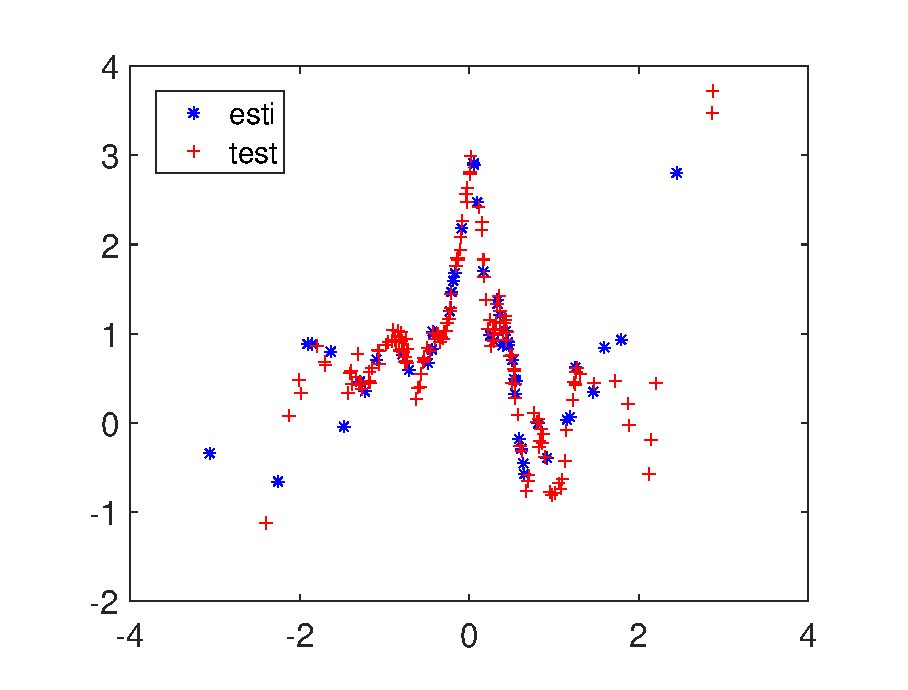
\includegraphics[scale=0.35]{./fig/例子1.eps}
        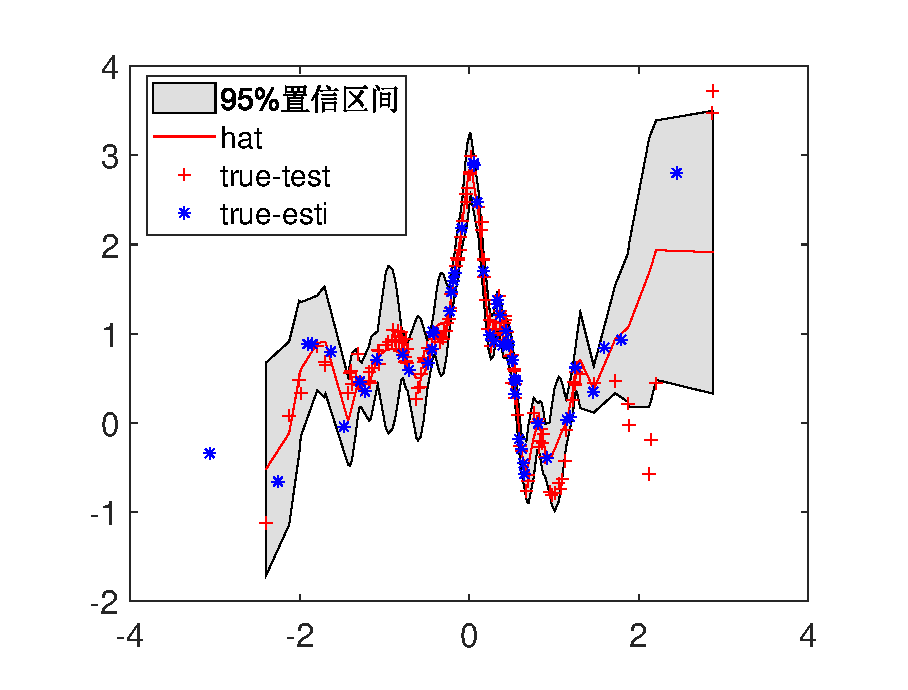
\includegraphics[scale=0.35]{./fig/例子2.eps}
        \caption{仿真}
    \end{figure}

    工具: Matlab + GPML ToolBox

    \monaco{meanfunc = \{@meanSum, \{@meanLinear, @meanConst\}\}; }

    \monaco{covfunc = \{@covMaterniso, 3\};}

\end{frame}

% 26
\begin{frame}{高斯过程回归模型应用 - 大气$CO_{2}$浓度预测}

    大气$CO_{2}$浓度预测取是《$GPML$》中的一个例子, 作者选取了1958年到2003年以月为间隔的545个数据(大气平均$CO_{2}$浓度)用于估计模型参数, 设计的模型协方差函数如下, 

    $$k_{1}(x,x')=\theta^{2}_{1}\mathrm{exp}\left(-\frac{(x-x')^{2}}{2\theta^{2}_{2}}\right)$$

    $$k_{2}(x,x')=\theta^{2}_{3}\mathrm{exp}\left(-\frac{(x-x')^{2}}{2\theta^{2}_{4}}-\frac{2sin^{2}(\pi(x-x'))}{\theta^{2}_{5}}\right)$$

    $$k_{3}(x,x')=\theta^{2}_{6}\left(1+\frac{(x-x')^{2}}{2\theta_{8}\theta^{2}_{7}}\right)^{-\theta_{8}}$$

    $$k_{4}(x_{p},x_{q})=\theta^{2}_{9}\mathrm{exp}\left(-\frac{(x_{p}-x_{q})^{2}}{2\theta^{2}_{10}}\right)+\theta_{11}\delta_{pq}$$

    $$k(x,x')=k_{1}(x,x')+k_{2}(x,x')+k_{3}(x,x')+k_{4}(x,x')$$

    % \vspace{-1ex}
    % \begin{figure}[H]
    %     \centering
    %     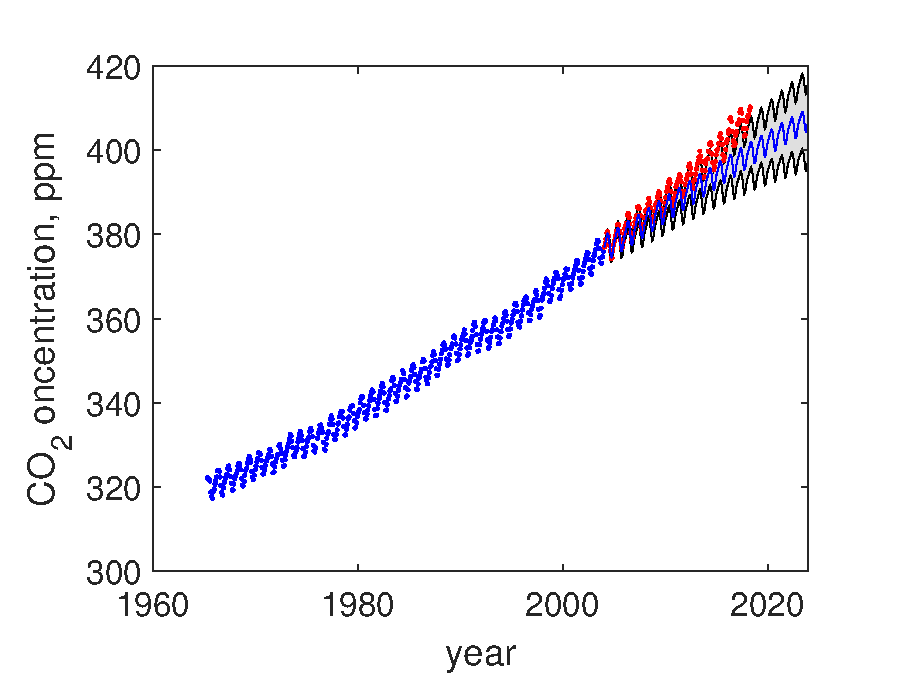
\includegraphics[scale=0.4]{./fig/co2.eps} 
    %     \caption{$大气CO_{2}$浓度预测}
    % \end{figure}
\end{frame}

% 注意这里插入eps之前一定要有文字 否则图片的坐标刻度会变粗!!!
% 27
\begin{frame}{高斯过程回归模型应用 - 大气$CO_{2}$浓度预测}
    预测结果,
    \vspace{-1ex}
    \begin{figure}[H]
        \centering
        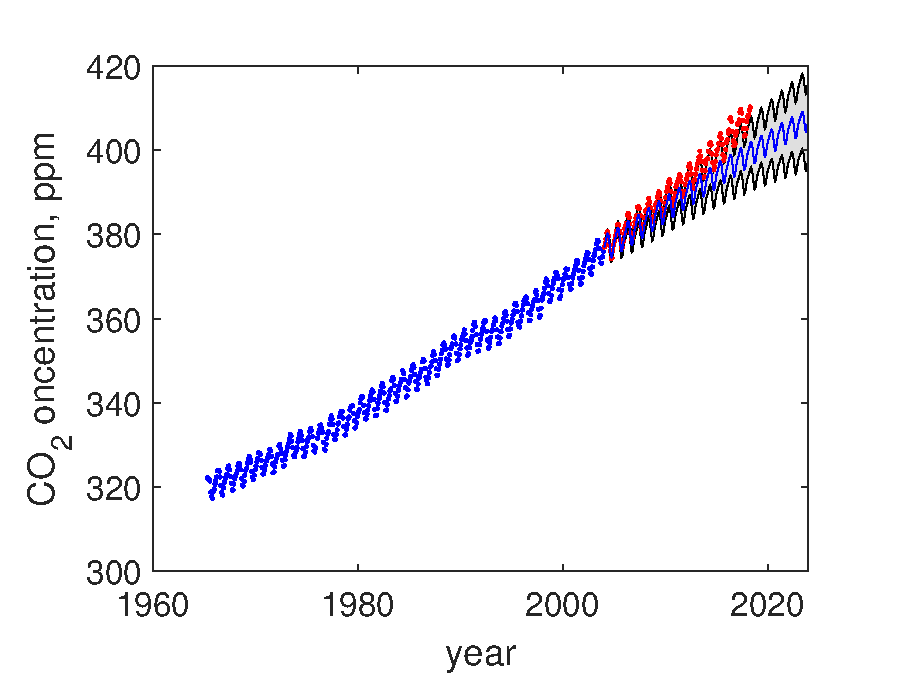
\includegraphics[scale=0.5]{./fig/co2.eps} 
        \caption{$大气CO_{2}$浓度预测}
    \end{figure}
\end{frame}

% 28
% 注意使用bibtex的编译方案
\begin{frame}[allowframebreaks]{参考}
    \nocite{rasmussen2006gaussian}
    \nocite{Rasmussen2017}
    \nocite{zhangjiangfan2017}
    \nocite{Durrande2017}

    \bibliography{bibcite}
    % \bibliographystyle{abbrv}
    \vspace{-0.5ex}
    ...
\end{frame}

%------------------------  尾页  ------------------------------

% 29
\begin{frame}[standout]
    Questions?
\end{frame}

% 30
\begin{frame}{}
    \begin{center}
        \textbf{\textsc{\erhao Thank you!}}
    \end{center}
\end{frame}